\section*{mechanika tlakové desky}
\addcontentsline{toc}{subsection}{mechanika tlakové desky}

Indukčně snímaná tlaková deska, funguje díky čtyřem cívkám, na desce plošných spojů, které mění svojí indukčnost podle vzdálenosti snímané desky, terčíku.
Z tohoto důvodu se terčík při používání naklání, čímž zároveň mění svojí vzdálenost od jednotlivých cívek. Z toho také plyne nutnost uložit terčík
částečně volně. Terčík je proto od snímací desky oddělen pružnou vložkou, která je zároveň předepnuta pomocí nažehlovací folie která kryje přední 
stranu dveří, a spojuje terčík s čelní krycí deskou. Díky nažehlovací folii je také přední část dveří voděodolné.

\begin{figure}[htbp]
    \centering
    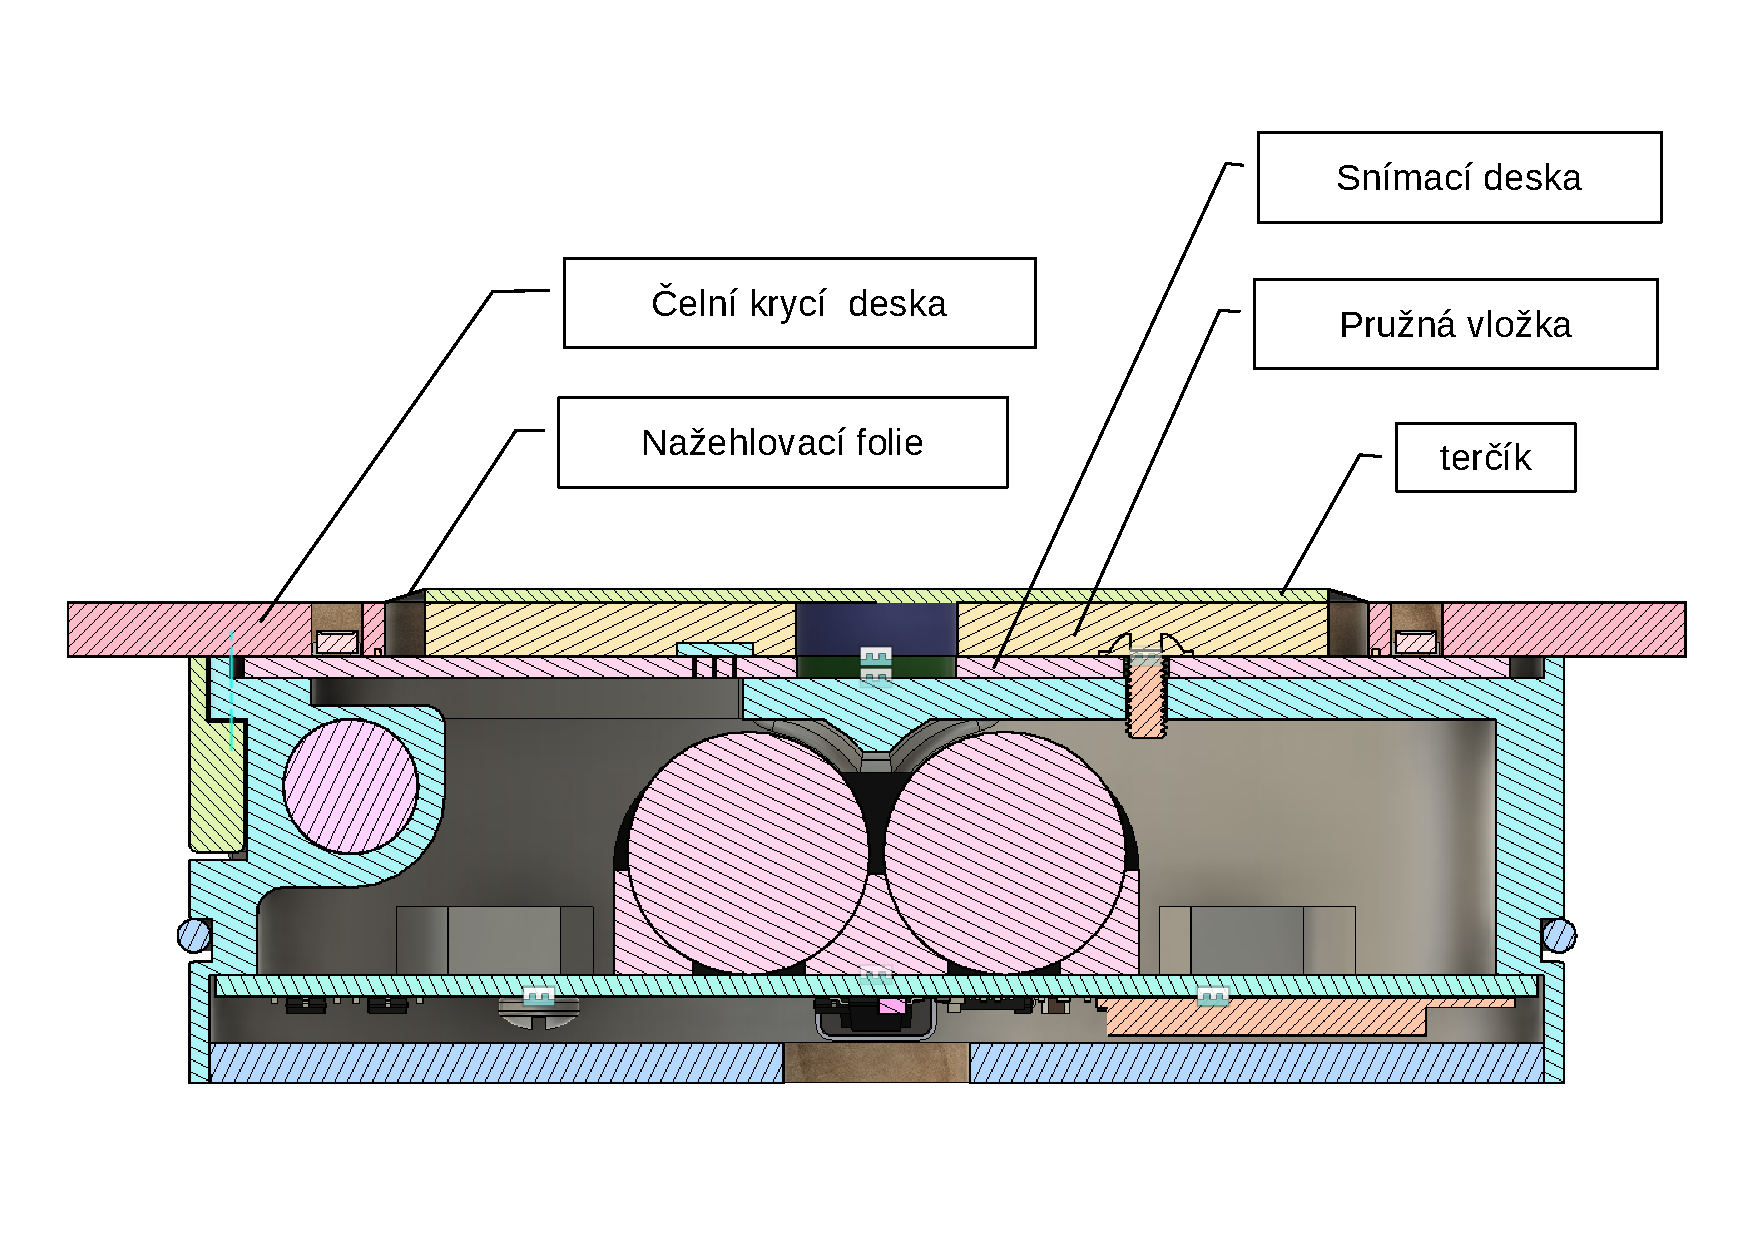
\includegraphics[width=\textwidth]{kapitoly/obrazky/tlakova_deska/rez_po_ose.pdf}
    \label{fig:M1}
\end{figure}

Tlaková deska zárově počítá s možností působení síli o velikosti až 100N, což samozřejmě zároveň znamená že tělo dveří tomuto zatížení musí odolat.
Vzhledem k tomu že nemám možnost vyrobit tělo z kovu, a jsem odkázán na 3D tisk a laserovou řezačku, a zároveň chci mít dveře co možná nejmenší,
musel jsem napočítat kritické části napřesno. Z tohoto důvodu jsem v programu Fusion 360, ve kterém jsem trezor vyvíjel,
dělal simulace, kterou zde přikládám. 

Jako materiál jsem v první fázi zvolil standardní fotopolimer pro tiskárny typu SLA, s pevností v tahu 46 až 67 MPa.
V budoucnu bych ale chtěl tělo odlévat z nějakého houževnatého polyuretanu, aby se zlevnila výroba a zároveň stoupla odolnost.

\begin{figure}[htbp]
    \centering
    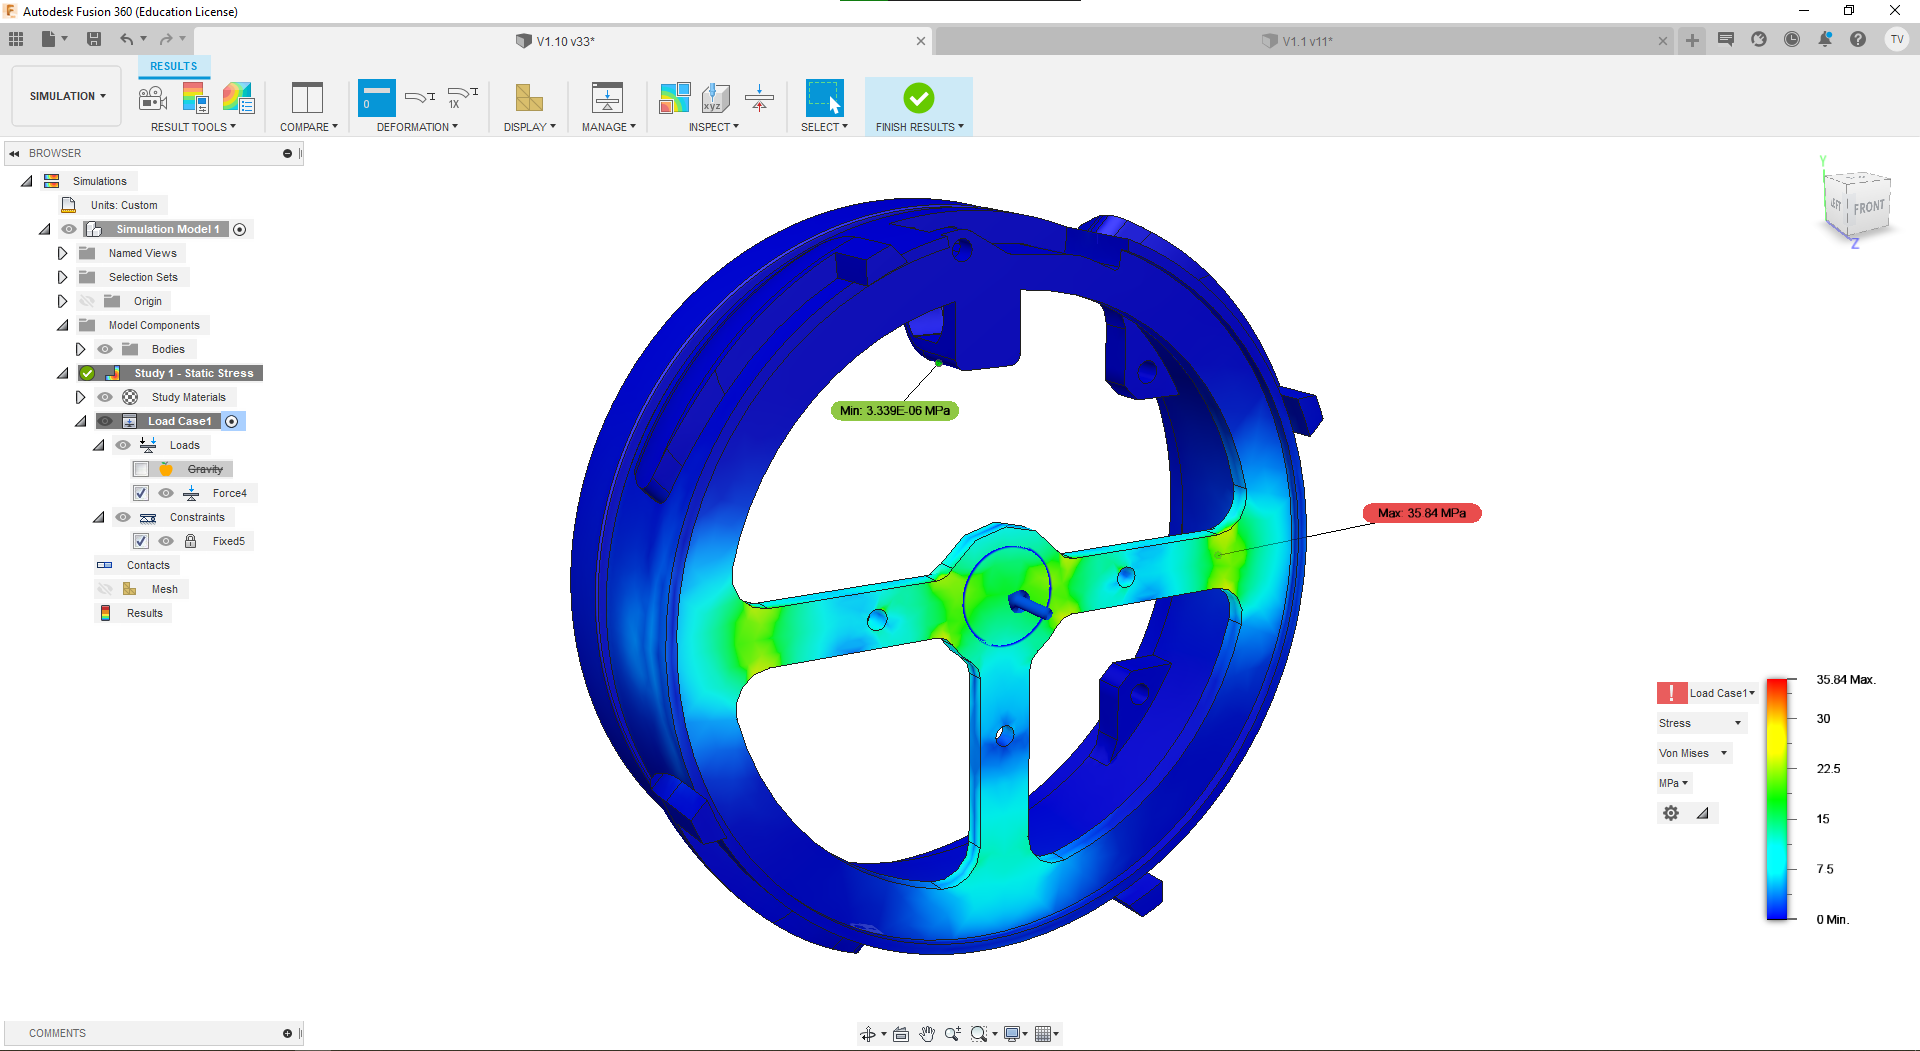
\includegraphics[width=\textwidth]{kapitoly/obrazky/tlakova_deska/simulace/F100N,primo,uprostred,pohled_zepredu.png}
    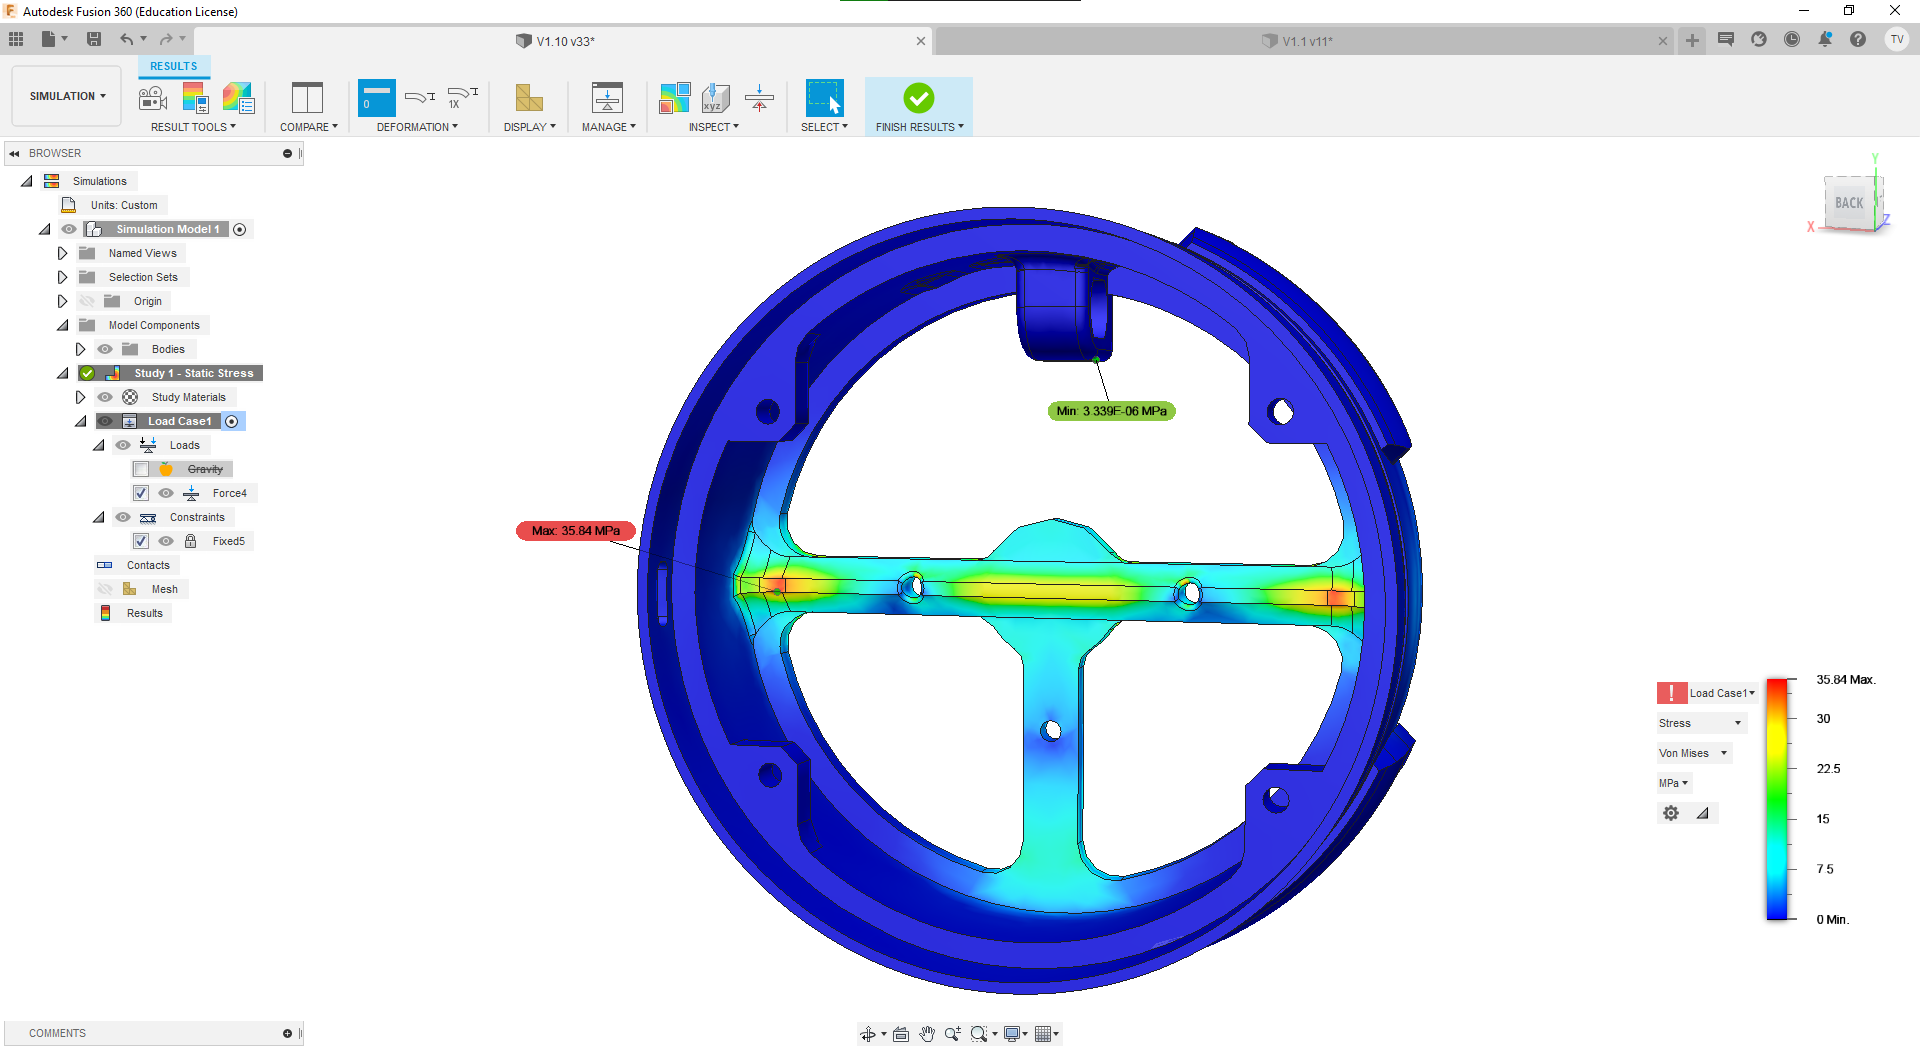
\includegraphics[width=\textwidth]{kapitoly/obrazky/tlakova_deska/simulace/F100N,primo,uprostred,pohled_zezadu.png}
    \label{fig:M1}
\end{figure}


\newpage